% generated by scripts/pkl_to_latex.py
% source PKL : tscan_v1_L6_Ne6_U5_mode-uniform_nmin2_solver-gcg_full_restarts10_iter300_kmax5_tol1em09_t0.05to2_N21-32c2aa6cb1ca.pkl
% scan type  : tscan
% state      : gs
% requires   : \usepackage{pgfplots} \pgfplotsset{compat=1.18}
% colours match the matplotlib PDF (tab10 cycle)
\definecolor{gmeC0}{HTML}{1F77B4}
\definecolor{gmeC1}{HTML}{FF7F0E}
\definecolor{gmeC2}{HTML}{2CA02C}
\definecolor{gmeC3}{HTML}{D62728}
\definecolor{gmeC4}{HTML}{9467BD}
\definecolor{gmeC5}{HTML}{8C564B}
\definecolor{gmeC6}{HTML}{E377C2}
\definecolor{gmeC7}{HTML}{17BECF}

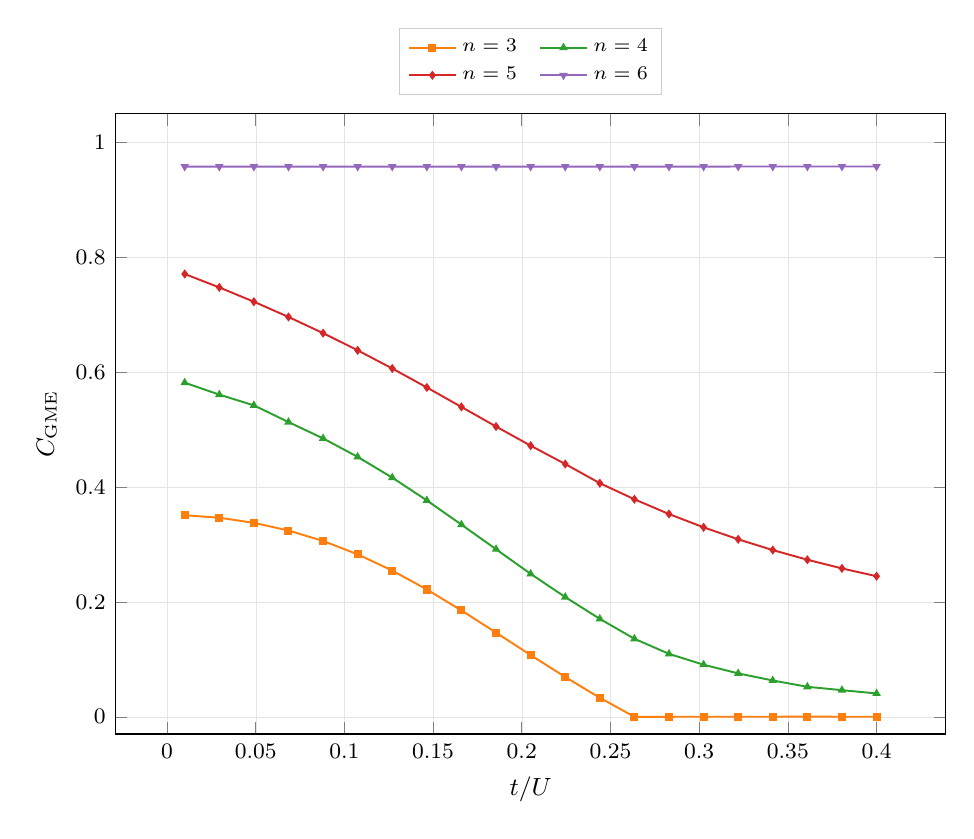
\begin{tikzpicture}
  \begin{axis}[
    width=\columnwidth,
    height=0.78\columnwidth,
    xlabel={$t/U$},
    ylabel={$C_{\mathrm{GME}}$},
    grid=both,
    grid style={line width=.1pt, draw=gray!20},
    tick label style={font=\footnotesize\rmfamily, /pgf/number format/fixed},
    label style={font=\small\rmfamily},
    scaled ticks=false,
    legend style={font=\scriptsize\rmfamily, draw=gray!40, at={(0.5,1.03)}, anchor=south, /tikz/every even column/.append style={column sep=6pt}},
    legend cell align={left},
    legend columns=2,
    ymin=-0.03,
    ymax=1.05,
  ]
    \addplot[color=gmeC1, mark=square*, mark size=1.1pt, line width=0.7pt] coordinates {
        (0.01,0.351113) (0.0295,0.346661) (0.049,0.33779) (0.0685,0.324382)
        (0.088,0.306192) (0.1075,0.28296) (0.127,0.254651) (0.1465,0.221721)
        (0.166,0.185212) (0.1855,0.146603) (0.205,0.107502) (0.2245,0.069328)
        (0.244,0.03313) (0.2635,0.000029) (0.283,0.000042) (0.3025,0.000084)
        (0.322,0.000129) (0.3415,0.000059) (0.361,0.000473) (0.3805,0.000034)
        (0.4,0.000144)
    };
    \addlegendentry{$n=3$}
    \addplot[color=gmeC2, mark=triangle*, mark size=1.1pt, line width=0.7pt] coordinates {
        (0.01,0.581864) (0.0295,0.561051) (0.049,0.542356) (0.0685,0.513282)
        (0.088,0.484864) (0.1075,0.452658) (0.127,0.4165) (0.1465,0.376836)
        (0.166,0.334615) (0.1855,0.291849) (0.205,0.248903) (0.2245,0.208551)
        (0.244,0.170548) (0.2635,0.13588) (0.283,0.109605) (0.3025,0.090686)
        (0.322,0.07559) (0.3415,0.063252) (0.361,0.052247) (0.3805,0.04639)
        (0.4,0.040674)
    };
    \addlegendentry{$n=4$}
    \addplot[color=gmeC3, mark=diamond*, mark size=1.1pt, line width=0.7pt] coordinates {
        (0.01,0.771122) (0.0295,0.747715) (0.049,0.722847) (0.0685,0.696298)
        (0.088,0.668134) (0.1075,0.638206) (0.127,0.606564) (0.1465,0.573493)
        (0.166,0.539562) (0.1855,0.505519) (0.205,0.472173) (0.2245,0.440206)
        (0.244,0.406823) (0.2635,0.37881) (0.283,0.353071) (0.3025,0.329935)
        (0.322,0.309109) (0.3415,0.290336) (0.361,0.273511) (0.3805,0.258419)
        (0.4,0.244811)
    };
    \addlegendentry{$n=5$}
    \addplot[color=gmeC4, mark=triangle*, mark size=1.1pt, mark options={rotate=180}, line width=0.7pt] coordinates {
        (0.01,0.958179) (0.0295,0.958179) (0.049,0.958179) (0.0685,0.95818)
        (0.088,0.958181) (0.1075,0.958183) (0.127,0.958187) (0.1465,0.958191)
        (0.166,0.958197) (0.1855,0.958204) (0.205,0.958211) (0.2245,0.95822)
        (0.244,0.958229) (0.2635,0.958239) (0.283,0.958249) (0.3025,0.958259)
        (0.322,0.95827) (0.3415,0.95828) (0.361,0.95829) (0.3805,0.9583)
        (0.4,0.95831)
    };
    \addlegendentry{$n=6$}
  \end{axis}
\end{tikzpicture}
